\documentclass[thesis.tex]{subfiles}

\begin{document}

\iffulldocument\else
	\chapter{KdV5}
\fi

\section{Periodic multi-pulse solutions}

In this section, we will prove the existence of periodic multi-pulse solutions to \eqref{genODE}. The existence of multi-pulse solution on $\R$ follows from \cite{SandstedeStrut}. An $n-$periodic solution to \eqref{genODE} is a periodic orbit which resembles $n$ well-separated copies of the primary pulse. The $n$ peaks are separated by distances $2X_0, 2X_1, \dots, 2X_{n-1}$, as shown in Figure \ref{fig:permultipulse}.

\begin{figure}[H]
\label{fig:permultipulse}
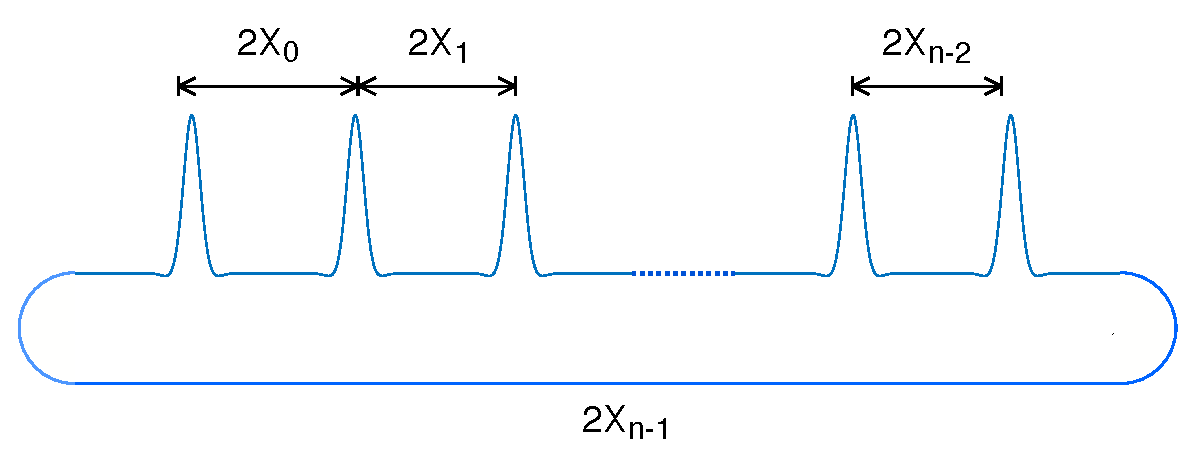
\includegraphics[width=10cm]{periodic/multipulseperiodic}
\caption{Periodic $n-$pulse solution.}
\end{figure} 

To prove existence of $n-$periodic solutions, we will use Lin's method. Rather than looking for these solutions as piecewise perturbations of the primary pulse solution $Q(x)$, we adapt the method in \cite{Sandstede1997} and take 
\[
U_i^\pm(x) = Q^\pm(x; \beta_i^\pm) + V_i^\pm(x)
\]
where $Q^\pm(0; \beta_i^\pm)$ paramaterizes the stable and unstable manifolds $W^s(0)$ and $W^u(0)$ near $Q(0)$ and $V_i^\pm$ is a small remainder term. In other words, we use the parameters $\beta_i^\pm$ to break the homoclinic orbit $Q(x)$.

We proceed as follows. First, we write $W^u(0)$ and $W^s(0)$ as graphs over their tangent spaces near $Q(0)$. Following \cite{Sandstede1997}, we can parameterize the unstable and stable manifolds near $Q(0)$ by the smooth functions $Q^-(\alpha, \beta^-)$ and $Q^+(\alpha, \beta^+)$, where $\alpha \in \R$, $\beta^\pm \in Y^\pm$ and these functions are chosen so that $Q^+(\alpha, 0) - Q^-(\alpha, 0) \in Z$. Note that $Q^+(0, 0) = Q^-(0, 0) = Q(0)$. We will always take $\alpha = 0$. Using this parameterization, let
\begin{align*}
Q^-(x; \beta^-) && x \leq 0 \\
Q^+(x; \beta^-) && x \geq 0
\end{align*}
be the unique solutions to \eqref{genODE} on $\R^\pm$ with initial conditions $Q^\pm(0, \beta^\pm)$ at $x = 0$. Since these initial conditions are on the unstable and stable manifolds (respectively), they decay exponentially (in the appropriate direction) with rate $\alpha_0$.

We will look for a $n-$periodic solution $U$ to \eqref{genODE} which is piecewise of the form
\begin{equation}\label{Upiecewise}
\begin{aligned}
U_i^-(x) &= Q^-(x; \beta_i^-) + V_i^-(x) && x \in [-X_{i-1}, 0] \\
U_i^+(x) &= Q^+(x; \beta_i^+) + V_i^+(x) && x \in [0, X_i]
\end{aligned}
\end{equation}
where $i = 0, \dots, n-1$, and the subscripts $i$ are taken $\mod n$ since we are on a perioidic domain. The periodic $n-$pulse consists of these $2n$ pieces spiced together end-to-end. Essentially, we are writing $U$ in terms of $2n$ parameters $\beta_i^\pm$, representing initial conditions on the unstable and stable manifolds, and $2n$ remainder functions $V_i^\pm(x)$. Since the initial conditions of $Q^\pm(x; \beta_i^\pm)$ are in $\R Q'(0) \oplus Y^\pm$, we can choose $V_i^\pm(x)$ with initial conditions
\begin{align*}
V_i^-(0) &\in Z \oplus Y^- \\
V_i^+(0) &\in Z \oplus Y^+
\end{align*}

Since we are looking for a continuous solution, we require the functions $U_i^\pm(x)$ to match at each of the $2n$ boundaries between intervals. Thus we need to solve the following system of equations
\begin{align}
(U_i^\pm)' - F(U_i^\pm) &= 0 \label{exsystem1} \\
U_i^+(X_i) - U_{i+1}^-(-X_i) &= 0 \label{exsystem2} \\
U_i^+(0) - U_i^-(0) &= 0 \label{exsystem3}
\end{align}
where $i = 0, \dots, n-1$. Using Lin's method, we will show that we can find a unique piecewise solution $U_i^\pm$ satisfying \eqref{exsystem1} and \eqref{exsystem2}. This solution will have $n$ jumps at $x = 0$, which must be in the direction of $\Psi(0)$. We will derive expressions for these jumps. A periodic multipulse solution exists if and only if these $n$ jumps are all 0.

In order to state the existence theorem for periodic multi-pulse solutions, we will adopt a convenient parameterization with a built-in scaling parameter rather than specify these solutions in terms of the lengths $X_i$. As in \cite{SandstedeStrut}, define the two sets
\begin{align}
\mathcal{R} &= \left\{ \exp\left(-\frac{m \pi}{\rho}\right) : m \in \N_0 \right\} \cup \{ 0 \}  \\
\mathcal{B} &= \left\{ \exp\left(-\frac{m \pi}{\rho}\right) : m \in \N_0 \right\} \label{setB}
\end{align}
where $\rho = \beta_0 / \alpha_0$. We note that $\mathcal{R}$ is a complete metric space. We will describe a periodic multi-pulse using the following four sets of parameters. 

\begin{enumerate}[(i)]
\item A integer $n \geq 2$, which is the number of pulses.
\item A scaling parameter $r \in \mathcal{R}$.
\item A sequence of $n$ baseline length parameters $\{ b_0^0, \dots, b_{n-1}^0 \}$, where $b_j^0 \in \mathcal{B}$.
\item A phase parameter $\theta \in [-\arctan \rho, \pi - \arctan \rho)$.
\end{enumerate}
The pulse distances $X_i$ are be determined by these parameters. We prove the existence of periodic multi-pulse solutions to \eqref{genODE} in the following theorem. The existence result requires that the scaling parameter $r$ be sufficiently small, which means that the individual pulses must be well-separated.

\begin{theorem}[Existence of $n$-periodic solutions]\label{perexist}
Assume Hypotheses \ref{Ehyp}, \ref{Hhyp}, \ref{hypeqhyp}, \ref{Qexistshyp}, and \ref{H0transversehyp}. Let $Q(x)$ be a transversely constructed, symmetric primary pulse solution to \eqref{genODE}. Choose
\begin{itemize}
\item An integer $n \geq 2$ 
\item A sequence of $n$ baseline length parameters $\{ b_0^0, \dots, b_{n-1}^0 \}$, where 
\[
b_j^0 = \exp\left(-\frac{m_j \pi}{\rho}\right) \in \mathcal{B}
\]
and at least one of the $b_j^0$ is 1. Without loss of generality, take $b_{n-1}^0 \leq b_j^0$ (equivalently, $m_{n-1} \geq m_j$) for $j = 0, \dots, n-2$.
\item A phase parameter $\theta \in [-\arctan \rho, \pi - \arctan \rho)$.
\end{itemize}
with the restriction that for $j = 0, \dots, n-2$, neither of the following is true.
\begin{itemize}
\item $m_j = m_{n-1}$ and $\theta = -\arctan \rho$
\item $m_j = m_{n-1} - 1$ and $\theta = \pi-\arctan \rho$
\end{itemize}
Then there exists $r_0 > 0$ such that
\begin{enumerate}[(i)]

\item For any $r \in \mathcal{R}$ with $r < r_0$, there exists a unique $n$-periodic solution $U(x)$ to \eqref{genODE}. Bounds for the piecewise formulation \eqref{Upiecewise} are given in Lemma \ref{solvewithjumps}.

\item This solution is specified by the $n$ length parameters $b_j(r; m_j, \theta)$, where
\begin{align}
b_j(r; m_j, \theta) \rightarrow b^*_j(m_j, \theta) \text{ as } r \rightarrow 0
\end{align}
and
\begin{align}
b^*_j(m_j, 0) = b_j^0
\end{align}
Details on this parameterization are given in Lemma \ref{thetaparamlemma}

\item The individual pulses in $U(x)$ are separated by distances $2 X_0, \dots, 2 X_{n-1}$, where 
\begin{equation}\label{Xj}
X_j = -\frac{1}{2\alpha}\log(b_j(r; m_j, \theta) r) - \frac{\phi}{2 \beta} 
\end{equation}
and $\phi$ is a constant.

\item The domain has length $2X$, where $X = X_0 + \dots + X_{n-1}$ and is given by
\begin{align}
X = \frac{1}{2\alpha} \left(n |\log r| + |\log(b_0(r; m_0, \theta) \cdots b_{n-1}(r; m_{n-1}, \theta))| \right) - \frac{n \phi}{2 \beta}
\end{align}

\end{enumerate}
\end{theorem}

If one of the baseline length parameters $b_j^0$ is small (i.e. one of the distances $X_j$ is large), the periodic $n-$pulse ``resembles'' the $n-$pulse on the real line. Without loss of generality, since we are on a periodic domain, we will choose $b_{n-1}^0$ to be small. In the next theorem, we will prove a uniform existence result. To do this, we will choose only the first $n-1$ baseline length parameters; we will allow the final baseline length parameter and the phase parameter to vary. 

\begin{theorem}\label{unifperexist}
Assume Hypotheses \ref{Ehyp}, \ref{Hhyp}, \ref{hypeqhyp}, \ref{Qexistshyp}, and \ref{H0transversehyp}. Let $Q(x)$ be a transversely constructed, symmetric primary pulse solution to \eqref{genODE}. Choose
\begin{itemize}
\item An integer $n \geq 2$ 
\item A sequence of $n-1$ baseline length parameters $b_0^0, \dots, b_{n-2}^0$, where $b_j^0 \in \mathcal{B}$ and at least one of the $b_j^0$ is 1.
\end{itemize}
Then there exists $r_1 > 0$ and $b^* \in \mathcal{B}$ such that for any $r < r_1$, $b_{n-1}^0 \in \mathcal{B}$ with $b_{n-1}^0 \leq b^*$, and $\theta \in [-\arctan \rho, \pi - \arctan \rho)$, there exists a unique $n$-periodic solution $U(x)$ to \eqref{genODE}. This solution is the same as the one from Theorem \ref{perexist}.
\end{theorem}

Finally, we show that for the the family of $2-$periodic pulse, there is a pitchfork bifurcation in which solutions with unequal pulse distances bifurcate off of solutions with equal pulse distances. Note that in this case we adopt a different parameterization.

\begin{theorem}\label{2pulsebifurcation}
Assume Hypotheses \ref{Ehyp}, \ref{Hhyp}, \ref{hypeqhyp}, \ref{Qexistshyp}, and \ref{H0transversehyp}. Let $Q(x)$ be a transversely constructed, symmetric primary pulse solution to \eqref{genODE}. For every $M \in \N$ there exists $r_0 > 0$ such that for every $r \in \mathcal{R}$ with $r < r_0$, the following is true.
\begin{enumerate}[(i)]
	\item For every $\theta \in [0, \pi)$, there is a unique 2-periodic solution with equal length parameters 
	\[
	b_0(\theta) = b_1(\theta) = e^{-\frac{1}{\rho}\theta}
	\]
	\item For every $s \in [0, M]$, there is a unique 2-periodic solution with unequal length parameters
	\[
	(\tilde{b}_0, \tilde{b}_1) = (\tilde{b}_0(s, r), \tilde{b}_1(s, r))
	\]
	where
	\[
	\tilde{b}_1(s, 0) = e^{-\frac{1}{\rho}(\arctan \rho + s)}
	\]
	and
	\[
	\tilde{b}_0(s, 0) \rightarrow 1 \text{ as } s \rightarrow \infty
	\]
	\item These two branches meet at a pitchfork bifurcation at $(p_0(r), p_0(r))$, where $p_0(r) \rightarrow e^{-\frac{1}{\rho}\arctan \rho}$ as $r \rightarrow 0$. In terms of the two parameterizations,
	\[
	(\tilde{b}_0(0, r), \tilde{b}_1(0, r)) = (b_0(p_0(r)), b_1(p_0(r)) 
	= (p_0(r), p_0(r))
	\]
\end{enumerate}
\end{theorem}

\section{Spectral stability}

In the previous section, we proved existence of periodic multi-pulse solutions to \eqref{genODE}, which are bound states  for \eqref{genPDE}. To look at their spectral stability, we will study the spectrum of the linearization of \eqref{genPDE} about a bound state solution. Let $u^*(x)$ be an exponentially localized bound state solution to \eqref{genPDE} corresponding to parameter $c$. The PDE eigenvalue problem is given by 
\begin{equation}\label{PDEeig}
\partial_x H_c v = \lambda v
\end{equation}
where we recall from \eqref{PDElinearization} that $H_c = E''(\phi_c) + c$.

As in the previous section, we will use a spatial dynamics approach. To that end, we will write the PDE eigenvalue problem \eqref{PDEeig} as a first-order system in the standard way. Let $V(x) = (v(x), \partial_x v(x), \dots, \partial_x^{2m}v(x)) \in \R^{2m+1}$. Then we have the equivalent formulation
\begin{equation}\label{PDEeig2}
V'(x) = A(U^*(x))V(x) + \lambda B V(x)
\end{equation}
where $B$ is the $(2m+1) \times (2m+1)$ constant coefficient matrix
\begin{equation}\label{DefB}
B = \begin{pmatrix}0 & 0 & 0 & 0 & 0 \\0 & 0 & 0 & 0 & 0 \\  & 
\vdots & & \vdots & \\0 & 0 & 0 & 0 & 0 \\1 & 0 & 0 & 0 & 0 \end{pmatrix} 
\end{equation}

Since $u^*(x)$ is exponentially localized, $A(U^*(x))$ is exponentially asymptotic to the constant coeffient matrix $A(0)$. The following lemma describes the eigenvalues and kernel of $A(0)$.

\begin{lemma}\label{eigA0lemma}
The following hold concerning the eigenvalues of $A(0)$.
\begin{enumerate}[(i)]
\item $A(0)$ has a simple eigenvalue at 0 and a quartet of eigenvalues at $\pm \alpha_0 \pm \beta_0 i$. For any other eigenvalue $\nu$ of $A(0)$, $|\text{Re }\nu| > \alpha_0$.
\item We can find eigenvectors $V_0$ and $W_0$ of $A(0)$ and $-A^*(0)$ corresponding to the simple eigenvalue 0 with $\langle V_0, W_0 \rangle = 1$.
\item The projection on the kernel of $A(0)$ is given by
\begin{equation}\label{projkernelA0}
P_{\ker A(0)} = \langle W_0, \cdot \rangle V_0
\end{equation}
\end{enumerate} 
\end{lemma}

Since $A(0)$ is not hyperbolic, the results of \cite{Sandstede1998} do not apply. Let $W^s(0)$, $W^u(0)$, and $W^c(0)$ be the stable, unstable, and center manifolds of the equilibrium at 0. (These are not the same as in the previous section, but we will retain the notation for convenience). By reversibility, $\dim W^s(0) = m$ and $\dim W^u(0) = m$. The center manifold $W^c(0)$ is one-dimensional.

Let $Q(x) = (q(x), \partial_x q(x), \dots, \partial_x^{2m} q(x))$, where $q(x)$ is the symmetric primary pulse solution from Hypothesis \ref{Qexistshyp}. (We note that $Q(x) \in \R^{2m+1}$ here, so it has one additional component compared to $Q(x)$ in that section; for convenience, we keep the same notation since it represents the same bound state solution $q(x)$ to \eqref{genPDE}). The variational and adjoint variational equations associated with \eqref{PDEeig2} are
\begin{align}
V'(x) = A(Q(x)) V(x) \label{vareq2} \\
W'(x) = -A(Q(x))^* W(x) \label{adjvareq2}
\end{align}

Since $(\partial_x H_c)(\partial_x q) = 0$, it follows that $Q'(x)$ is an exponentially localized solution to the variational equation \eqref{vareq2}, i.e. 
\begin{equation}\label{Qprimevarsol}
(Q'(x))' = A(Q(x))Q'(x)
\end{equation}
Since $(H_c \partial_x)(-\partial_c q) = \partial_x q$, we also have
\begin{equation}\label{Qprimevarsol}
(Q_c(x))' = A(Q(x))Q_c(x) + BQ'(x)
\end{equation}
where $Q_c(x) = (\partial_c q(x), \partial_x \partial_c q(x), \dots, \partial_x^{2m}\partial_c q(x))$.

Since $Q(x)$ is exponentially localized, it cannot involve the center manifold $W^c(0)$, thus it must lie in the intersection of the stable and unstable manifolds. In particular, this implies that $\R Q'(0) \subset T_{Q(0)}W^s(0) \cap T_{Q(0)}W^u(0)$. It follows from \eqref{H0transversehyp} that these are actually equal, which we state in the following lemma.

\begin{lemma}\label{nondegenlemma}
We have the nondegeneracy condition
\begin{equation}\label{nondegen2}
T_{Q(0)}W^s(0) \cap T_{Q(0)}W^u(0) = \R Q'(0)
\end{equation}
\end{lemma}

Using the nondegeneracy condition \eqref{nondegen2}, we can decompose the tangent spaces of the stable and unstable manifolds at $Q(0)$ as
\begin{align*}
T_{Q(0)}W^s(0) &= \R Q'(0) \oplus Y^+ \\
T_{Q(0)}W^u(0) &= \R Q'(0) \oplus Y^- \\
\end{align*}
Since $\dim \R Q'(0) \oplus Y^+ \oplus Y^- = 2m-1$, there are two remaining directions needed in order to span $\R^{2m+1}$. To find these, we use the following two lemmas regarding solutions to \eqref{vareq2} and \eqref{adjvareq2}.

\begin{lemma}\label{varsolutions}
There exists a bounded solution $V^c(x)$ to \eqref{vareq2} such that 
\begin{equation}
V^c(x) \rightarrow V_0 \text{ as }|x| \rightarrow \infty
\end{equation}
where $V_0$ is the eigenvector of $A(0)$ corresponding to the simple eigenvalue 0. $V^c$ is symmetric with respect to the standard reversor operator $R$, i.e. $V^c(-x) = R V^c(x)$.
\end{lemma}

\begin{lemma}\label{adjsolutions}
There exist exactly two linearly independent, bounded solutions $\Psi(x)$ and $\Psi^c(x)$ to \eqref{adjvareq2}.
\begin{enumerate}[(i)]
\item $\Psi(x)$ is exponentially localized, i.e. $e^{\alpha_0 |x|}\Psi(x)$ is bounded, and the last component of $\Psi(x)$ is $q(x)$. In addition, $\Psi(x)$ is symmetric with respect to the standard reversor operator $R$, i.e. $\Psi(-x) = R \Psi(x)$. 
\item $\Psi_c(x)$ is bounded, the last component of $\Psi^c(x)$ is $1$, $\Psi^c(-x) = R \Psi^c(x)$, and
\begin{equation}
\Psi^c(x) \rightarrow W_0 \text{ as }|x| \rightarrow \infty
\end{equation}
where $W_0$ is the eigenvector of $-A(0)^*$ corresponding to the simple eigenvalue 0. Furthermore, $\Psi^c = (-DF(Q(x)), 1)$, and we have
\[
\langle \Psi^c(x), Q'(x) \rangle = \langle \Psi^c(x), Q'(-x) \rangle = 0
\]
\end{enumerate}
Finally, $\Psi(0), \Psi^c(0) \perp \R Q'(0) \oplus Y^+ \oplus Y^-$.
\end{lemma}
 
Using Lemma \ref{nondegenlemma} and Lemma \ref{adjsolutions}, we can decompose $\R^{2m+1}$ as  
\begin{equation}
\R^{2m+1} = \R \Psi(0) \oplus \R \Psi^c(0) \oplus \R Q'(0) \oplus Y^+ \oplus Y^-
\end{equation}
where $\R \Psi(0) \oplus \R \Psi^c(0) \perp \R Q'(0) \oplus Y^+ \oplus Y^-$.

The final hypothesis concerns a higher order Melnikov integral. Before we consider that, we note that the standard Melnikov integral is 0, i.e. 
\begin{equation}\label{M1}
M_1 = \int_{-\infty}^\infty \langle \Psi(x), B Q'(x) \rangle =
\int_{-\infty}^\infty q(x) \: \partial_x q(x) 
= \langle q(x), \partial_x q(x) \rangle_{L^2(\R)} = 0
\end{equation}
since the last component of $\Psi(x)$ is $q(x)$ by Lemma \ref{adjsolutions}, and $q(x)$ is an even function. We take the following hypothesis regarding a higher order Melnikov integral.
\begin{hypothesis}\label{Melnikov2hyp}
The following higher order Melnikov integral is nonzero.
\begin{equation}\label{M2}
M_2 = \int_{-\infty}^\infty \langle \Psi(x), B Q_c(x) \rangle dx =
\int_{-\infty}^\infty q(x) q_c(x) dx \neq 0
\end{equation}
\end{hypothesis}
In applications such as KdV5, numerics suggests that Hypothesis \ref{Melnikov2hyp} is satisfied.

Let $q_{np}(x)$ be a periodic $n-$pulse solution constructed according to Theorem \ref{perexist}. To solve the PDE eigenvalue problem \eqref{PDEeig2} for the linearization about $q_{np}(x)$, we will use Lin's method to construct an eigenfunction $V(x)$ as a small perturbation of a piecewise linear combination of $Q'(x)$ and $Q_c(x)$. For $X_m = \min\{X_0, \dots, X_{n-1} \}$ sufficiently large and $\lambda$ sufficiently small, Lin's method provides a unique function $V(x)$ which solves \eqref{PDEeig2}, but in general $V(x)$ has $n$ jump discontinuities; it is a true eigenfunction if all of these jumps are 0. Lin's method also yields a formula for these jumps. Finding the eigenvalues $\lambda$ then amounts to solving the $n$ jump conditions.

To use Lin's method, we rewrite the PDE eigenvalue problem \eqref{PDEeig2} as
\begin{equation}\label{PDEeig3}
V' = A(U^*(x); \lambda)V 
\end{equation} 
where $A(U^*(x); \lambda) = A(U^*) + \lambda B$. For $\lambda = 0$, the asymptotic matrix $A(0; 0)$ has a simple eigenvalue at 0. The next lemma states that for small $\lambda$, $A(0; \lambda)$ has a small eigenvalue $\nu(\lambda)$ near 0.

% nu(lambda) lemma
\begin{lemma}\label{nulambdalemma}
There exists $\delta_0 > 0$ such that for $|\lambda| < \delta_0$, the asymptotic matrix $A(\lambda)$ has a simple eigenvalue $\nu(\lambda)$. $\nu(\lambda)$ is smooth in $\lambda$, $\nu(0) = 0$, and for $|\lambda| < \delta_0$,
\begin{equation}\label{nulambda}
\nu(\lambda) = \frac{1}{c} \lambda + \mathcal{O}(|\lambda|^3)
\end{equation}
In addition,
\begin{enumerate}[(i)]
\item $\nu(-\lambda) = -\nu(\lambda)$, i.e. $\nu(\lambda)$ is an odd function 
\item If $\lambda$ is pure imaginary, $\nu(\lambda)$ is also pure imaginary
\item The corresponding eigenvector to $\nu(\lambda)$ is $V_0(\lambda)$ which is smooth in $\lambda$ and has Taylor expansion
\begin{equation}\label{V0expansion}
V_0(\lambda) = V_0 + \lambda \tilde{V}_0 + \mathcal{O}(\lambda^2),
\end{equation}
Furthermore, $V_0(-\lambda) = R V_0(\lambda)$ and $\tilde{V}_0 = -R \tilde{V}_0$, where $R$ is the standard reversor operator.
\end{enumerate}

Similarly, the adjoint asymptotic matrix $-A(\lambda)^*$ has an eigenvalue $-\overline{\nu(\lambda)}$ with corresponding eigenvector $W_0(\overline{\lambda})$, both of which are smooth in $\overline{\lambda}$. $W_0(\overline{\lambda})$ has Taylor expansion
\begin{equation}\label{W0expansion}
W_0(\lambda) = W_0 + \overline{\lambda} \tilde{W}_0 + \mathcal{O}(\overline{\lambda}^2),
\end{equation}
with symmetry propterties $W_0(-\overline{\lambda}) = R W_0(\overline{\lambda})$ and $\tilde{W}_0 = -R \tilde{W}_0$
\end{lemma}

We can now state the main theorem of the section, which gives us a condition for $\lambda$ to be an eigenvalue of \eqref{PDEeig3}. This theorem is analagous to \cite[Theorem 2]{Sandstede1998}, with the matrix $A$ replaced by a block matrix.

% block matrix theorem
\begin{theorem}\label{blockmatrixtheorem}
Assume Hypotheses \ref{Ehyp}, \ref{Hhyp}, \ref{hypeqhyp}, \ref{Qexistshyp}, and \ref{H0transversehyp}. Let $q_{np}(x)$ be a periodic $n-$pulse solution constructed according to Theorem \ref{perexist} with lengths $X_0, \dots, X_{n-1}$. Then there exists $\delta \leq \delta_0$ with the following property: there exists a bounded, nonzero solution $V$ of \eqref{PDEeig} for $|\lambda| < \delta$ if and only if the block matrix equation
\begin{equation}\label{blockeq}
\begin{pmatrix}
K(\lambda) + C_1 K(\lambda) + K_1(\lambda) & \tilde{A} + D_1 \\
\lambda M_\Psi \tilde{K}(\lambda) + C_2 K(\lambda) + K_2(\lambda) & A - \lambda^2 MI + D_2
\end{pmatrix}
\begin{pmatrix} c \\ d \end{pmatrix} = 0
\end{equation}
has a nontrivial solution, where 

\begin{enumerate}
\item The matrix $K(\lambda)$ is given by
\begin{equation}
K(\lambda) = 
\begin{pmatrix}
e^{-\nu(\lambda)X_1} & & & & & -e^{\nu(\lambda)X_0} \\
-e^{\nu(\lambda)X_1} & e^{-\nu(\lambda)X_2} \\
& -e^{\nu(\lambda)X_2} & e^{-\nu(\lambda)X_3} \\
& \ddots & \ddots & &&  \\
& & & & -e^{\nu(\lambda)X_{n-1}} & e^{-\nu(\lambda)X_0} 
\end{pmatrix}
\end{equation}
where $\nu(\lambda)$ is defined in Lemma \ref{nulambdalemma}. $\tilde{K}(\lambda)$ is the same matrix with all terms positive.

\item $A$ is the symmetric matrix
\begin{align}\label{Asymm}
A &= \begin{pmatrix}
-a_0 -a_1 & a_0 + a_1 \\
a_0 + a_1 & -a_0 - a_1
\end{pmatrix} && n = 2 \\
A &= \begin{pmatrix}
-a_{n-1} - a_0 & a_0 & & &  & a_{n-1}\\
a_0 & -a_0 - a_1 &  a_1 \\
& a_1 & -a_1 - a_2 &  a_2 \\
& \ddots & \ddots & \ddots \\
a_{n-1} & & & & a_{n-2} & -a_{n-2} - a_{n-1} \\
\end{pmatrix} && n > 2 \nonumber
\end{align}
where
\begin{align*}
a_i &= \langle \Psi(X_i), Q'(-X_i) \rangle
\end{align*}
$\tilde{A}$ is the same matrix with entries
\begin{align*}
\tilde{a}_i &= \langle \Psi^c(X_i), Q'(-X_i) \rangle
\end{align*}
and $||\tilde{A}|| = \mathcal{O}(e^{-\alpha X_m})$.

\item $M$ is the higher order Melnikov integral
\begin{align*}
M &= \int_{-\infty}^\infty \Psi(y) t(y) dy \\
\end{align*}
$M_\Psi$ WILL BE DEFINED ONCE WE FIGURE OUT WHAT IT IS.

\item The remainder terms are analytic in $\lambda$ and have uniform bounds
\begin{align*}
C_1 &= \mathcal{O}(e^{-(\alpha - \eta) X_m}(|\lambda| + e^{-\alpha X_m})) \\
D_1 &= \mathcal{O}((|\lambda| + e^{-\alpha X_m})^2) \\
C_2 &= \mathcal{O}(e^{-(\alpha - \eta) X_m}(|\lambda| + e^{-\alpha X_m})^2) \\
D_2 &= \mathcal{O}((|\lambda| + e^{-\alpha X_m})^3)
\end{align*}
where $\eta < \alpha_0/4$, $\alpha = \alpha_0 - \eta$, and $X_m = \min\{X_0, \dots, X_{n-1}\}$.

\item $K_1(\lambda)$ and $K_2(\lambda)$ are matrices where the nonzero terms of $K(\lambda)$ are multiplied by $\mathcal{O}(|\lambda| + e^{-\alpha X_m})$ and $\mathcal{O}(|\lambda| + e^{-\alpha X_m})^2$ (respectively). These are defined precisely in the proofs of Lemmas \ref{jumpcenteradj} and \ref{jumpadj}

\end{enumerate}
\end{theorem}

\section{Location of Eigenvalues}

We can use Theorem \ref{blockmatrixtheorem} to locate the eigenvalues of \eqref{PDEeig3}. Note that the matrix $A$ from Theorem \ref{blockmatrixtheorem} is symmetric, thus its eigenvalues are real. $A$ has an eigenvalues of 0 corresponding to eigenvector $(1, 1, \dots, 1)^T$. We will hypothesize that the eigenvalues of $A$ distinct. 

\begin{hypothesis}\label{Adistincteigs}
The eigenvalues of $A$ are given by $(0, \mu_1, \dots, \mu_{n-1})$, all of which are distinct.
\end{hypothesis}

This is not true in general. For example, if $n \geq 3$ and all the terms $a_i$ in $A$ are identical, $A$ is a circulant matrix and it is not hard to show that $A$ will have eigenvalues of algebraic multiplicity 2.

We expect to find eigenvalues near where the matrices $K(\lambda)$ and $A - \lambda^2 MI$ are singular. This happens at the following values of $\lambda$. 
\begin{itemize}
	\item $A - \lambda^2 M I$ is singular at $\lambda = 0$ (algebraic multiplicity 2) and 
	\[
	\lambda = \{ \pm r^{1/2} \sqrt{\tilde{\mu}_1/M}, \dots, \pm r^{1/2} \sqrt{\tilde{\mu}_{n-1}/M}\}
	\]
	where $\{0, r \tilde{\mu}_1, \dots, r \tilde{\mu}_{n-1}\}$ are the eigenvalues of $A$. 

	\item $K(\lambda)$ is singular at $\lambda = \pm \lambda^K(X,k)$ for integer $k$, where $\lambda(X, 0) = 0$ (algebraic multiplicity 1) and
	\begin{align}\label{lambdaXkapprox}
	\lambda^K(X,k) \approx c \frac{k \pi i }{X} 
	\end{align}
	Since 
	\[
	X = \frac{1}{2\alpha} (n |\log r| + |\log b_0 b_1 \cdots b_{n-1}| ) - \frac{n \phi}{2 \beta}
	\]
	we have
	\[
	\lambda^K(X,k) \approx C \frac{k i}{n |\log r|}
	\]
\end{itemize}  

For the analysis to work, we need to ensure that the nonzero singular points of these two matrices do not get too close. We have observed Krein bubbles numerically when interaction eigenvalues with negative Krein signature collide with ``essential spectrum'' eigenvalues of positive Krein signature. We make the following definition

\begin{definition}\label{epsilonballs}
A periodic $n-$pulse parameterized as in Theorem \ref{perexist} satisfies the \emph{$\epsilon-$ball condition} if the two sets of points 
\begin{itemize}
\item $\lambda = \pm r^{1/2} \sqrt{\tilde{\mu}_1/M}, \dots, \pm r^{1/2} \sqrt{\tilde{\mu}_{n-1}/M}$
\item $\lambda = \lambda^K(X,k)$ with $k$ nonzero integer and $|\lambda^K(X,k)| < \delta$
\end{itemize}
are separated by at least $\epsilon$, where
\[
\epsilon = \frac{r^{1/4}}{4X} = \mathcal{O} \left( \frac{r^{1/4}}{n |\log r| } \right)
\]
\end{definition}

The following lemma states that this condition can always be satisfied.

\begin{lemma}\label{epsilonballlemma}
Choose baseline length parameters $b_0^0, \dots, b_{n-1}^0$ and phase parameter $\theta$. Then there exists $r(b, \theta) \leq r_0$ such that for $r \leq r(b, \theta)$, the $\epsilon-$ball condition is satisfied.
\end{lemma} 

Although we can always choose sufficiently small $r$ so that the $\epsilon$-ball condition is satisfied, it is useful to retain this definition. The proof of Lemma \ref{epsilonballlemma} is constructive and guarantees that for all sufficiently small $r$, any purely imaginary interaction eigenvalues will always lie between 0 and the smallest nonzero ``essential spectrum'' eigenvalues. A 2-periodic pulse, for example, would give us the eigenvalue pattern

\begin{figure}[H]
\begin{center}
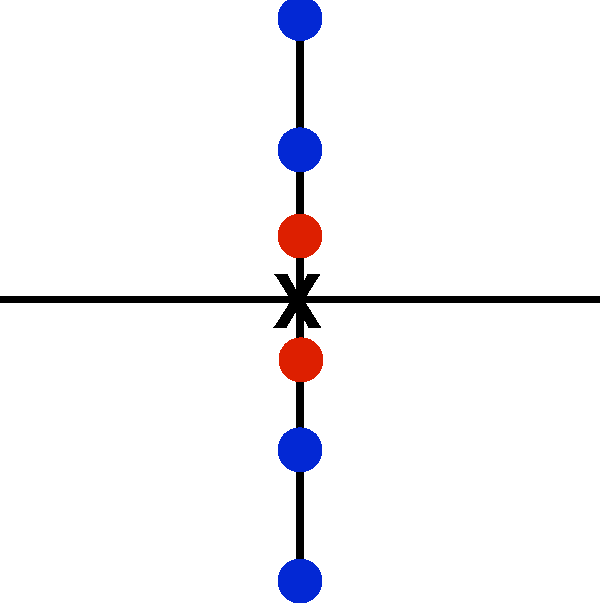
\includegraphics[width=4cm]{periodic/2pulseess}
\end{center}
\caption{Interaction eigenvalues in red, ``essential spectrum'' eigenvalues in blue.}
\end{figure}

We prefer not to restrict ourselves to this case for the following reason. Consider a $2-$periodic pulse with scaling parameter $r$, length parameters $b_0^0 = 1$ and $b_1^0 = \exp(-\pi m_1/\rho)$, and phase parameter $\theta = 0$ (for convenience). If the length parameter $b_1^0$ is sufficiently small (i.e. $m_1$ is sufficiently large), we can \emph{decrease} $b_1^0$ while keeping the same $r$. From Theorem \ref{unifperexist}, we get a whole family of $2-$periodic pulses this way. The domain length is $2X$, where
\[
X \approx C \Big( 2 |\log r| + |\log(b_0 b_1)| \Big)
\]
If we keep $r$ fixed and decrease $b_1^0$ (which decreases $b_1$), $X$ will grow, but the interaction eigenvalues will not change much. On the other hand, the ``essential spectrum'' eigenvalues will move towards the origin. This will cause an ``essential spectrum'' eigenvalue to pass through an interaction eigenvalue. It is unclear at present what happens when these eigenvalues cross, but we have observed Krein bubbles numerically. The $\epsilon-$ball condition gives us an upper bound on the size of these Krein bubbles.

With this out of the way, we can use the following theorem to locate the eigenvalues of \eqref{PDEeig} near the origin.

% eigenvalue location theorem

\begin{theorem}\label{locateeigtheorem}
Assume Hypotheses \ref{Ehyp}, \ref{Hhyp}, \ref{hypeqhyp}, \ref{Qexistshyp}, \ref{H0transversehyp}, \ref{Melnikov2hyp}, and \ref{Adistincteigs}. Let $q_{np}(x)$ be a periodic $n-$pulse solution constructed according to Theorem \ref{perexist} with scaling parameter $r \leq r_0$. Let $\delta > 0$ be defined as in Theorem \ref{blockmatrixtheorem}. Then the following are true.

\begin{enumerate}[(i)]

\item There is an eigenvalue at 0 with (at minimum) geometric multiplicity 2 and algebraic multiplicity 3. The eigenfunctions are the kernel eigenfunction $\partial_x q_{np}(x)$ from translation invariance; its generalized kernel eigenfunction $t_{np}(x)$; and a third kernel eigenfunction $v^c(x)$ which is bounded but does not decay exponentially.

\item There exists $r_1 \leq r_0$ such that for every $r \leq r_1$ for which the $\epsilon-$ball condition is satisfied, there are $n - 1$ pairs of interaction eigenvalues given by $\lambda = \pm \lambda^{\text{int}}_j(r)$ for $j = 1, \dots, n-1$, where
\begin{align*}
\lambda^{\text{int}}_j(r) = r^{1/2} \sqrt{\tilde{\mu}_j / M} + \mathcal{O}(r^{3/4})
\end{align*}
These interaction eigenvalue pairs are either real or purely imaginary, and the remainder term cannot move them off of the real or imaginary axis.

\item There exists $r_2 \leq r_1$ such that for every $r \leq r_2$ for which the $\epsilon-$ball condition is satisfied, there are pairs of purely imaginary ``essential spectrum'' eigenvalues given by $\lambda = \pm \lambda^{ess}(X,k; r)$ for every positive integer $k$ with $\frac{c \pi k}{X} < \delta$ (approximately $k < \delta n |\log r|$), where
\begin{equation}\label{lambdaess}
\lambda^{ess}(X, k; r) = c \frac{k \pi i }{X} \left( 1 + \mathcal{O}\left( \frac{1}{X} \right)\right) + \mathcal{O}\left( \frac{r^{1/2}}{X} \right)
\end{equation}
In terms of $r$ and the $b_j$, these are located at approximately
\begin{equation}\label{lambdaessr}
\lambda^{ess}(k; r) = C \frac{k \pi i }{n |\log r| + |\log (b_0 b_1 \cdots b_{n-1})|}  \left( 1 + \mathcal{O}\left( \frac{1}{n |\log r|} \right)\right) + \mathcal{O}\left( \frac{r^{1/2}}{n |\log r|} \right)
\end{equation}
The remainder terms cannot move these off of the imaginary axis.

\item For sufficiently small $r$, we have the following two eigenvalue counts.
\begin{itemize}
	\item There exists a small radius $\xi$ (which excludes the interaction eigenvalues and ``essential spectrum'' eigenvalues) such that there are exactly 3 eigenvalues inside the circle of radius $\xi$ in the complex plane. These must be the three eigenvalues from part (i).

	\item There are exactly $2n + 2 k_M + 1$ eigenvalues inside the circle of radius $\tilde{\delta}$ (which may be slightly smaller than $\delta$) in the complex plane, where $k_M$ is the largest positive integer $k$ such that $\lambda^K(k,X) < \tilde{\delta}$. 
\end{itemize}
If the $\epsilon-$ball condition is satisfied, there are no eigenvalues inside the circle of radius $\tilde{\delta}$ other than the ones already accounted for.
\end{enumerate}
\end{theorem}

If we can take one of the baseline length parameters $b_j^0$ to be small compared to the others, we are ``close to'' the situation on the real line. Since we are on a periodic domain, we can without loss of generality take $b_{n-1}^0$ to be small. Recall that the other baseline length parameters are given by
\begin{align*}
b_j^0 &= e^{-\frac{1}{\rho}m_j \pi} && j = 0, \dots, n-2
\end{align*}
for nonnegative integers $m_j$. In this case, the parity of the  integers $m_k$ determines the eigenvalue pattern.

\begin{theorem}\label{inteigsparity}
Assume Hypotheses \ref{Ehyp}, \ref{Hhyp}, \ref{hypeqhyp}, \ref{Qexistshyp}, \ref{H0transversehyp}, \ref{Melnikov2hyp}, and \ref{Adistincteigs}. Let $r_1$ and $b^*$ be as in Theorem \ref{unifperexist}. Choose an integer $n \geq 2$ and a sequence of $n-1$ baseline length parameters $b_0^0, \dots, b_{n-2}^0$, where $b_j^0 = \exp\left(-\frac{1}{\rho}m_j \pi\right) \in \mathcal{B}$. 

Then there exists $\tilde{r_1} \leq r_1$ and $\tilde{b}^* \in \mathcal{B}$ with $\tilde{b}^* \leq b^*$ such that for any $r \leq \tilde{r}_1$, $b_{n-1}^0 \in \mathcal{B}$ with $b_{n-1}^0 \leq \tilde{b}^*$, and $\theta \in [-\arctan \rho, \pi - \arctan \rho)$, we have the following result.

Let $r = \exp\left( -\frac{1}{\rho} m \pi \right)$, where $m$ is a nonnegative integer. If $M > 0$, then 
\begin{itemize}
\item If $m$ is even ($m$ is odd), there are $n_{\text{even}}$ purely imaginary (real) pairs of interaction eigenvalues.
\item If $m$ is even ($m$ is odd), there are $n_{\text{odd}}$ real (purely imaginary) pairs of interaction eigenvalues.
\end{itemize}
where $n_{\text{even}}$ is the number of even $\{m_0, \dots, m_{n-2}\}$ and $n_{\text{odd}}$ is the number of odd $\{m_0, \dots, m_{n-2}\}$. If $M < 0$, these are reversed.
\end{theorem}

Finally, we consider the case of the 2-periodic pulse. For the symmetric 2-periodic pulse (i.e. $b_0 = b_1$), the interaction eigenvalues are approximately
\[
\lambda^{\text{int}} = \pm C r^{1/2} e^{-\theta/2\rho} \sqrt{ \frac{1}{M} \left( \rho \cos \theta - \sin \theta \right) }
\]
which is 0 at $\theta = \arctan \rho$. At a point near there, there is a bifurcation in which a pair of real eigenvalues collides at 0 and then becomes a pair of purely imaginary eigenvalues. We can probably use a symmetry argument or something like that to show that this occurs for small $r$ at the actual pitchfork bifurcation point $\theta^*(r)$, where $\theta^*(0) = \arctan \rho$. This has been verified numerically.

\iffulldocument\else
	\bibliographystyle{amsalpha}
	\bibliography{thesis.bib}
\fi

\end{document}